%\documentclass[12pt,a4paper]{article}
%\usepackage[latin1]{inputenc}
%\usepackage{amsmath}
%\usepackage{amsfonts}
%\usepackage{amssymb}
%\usepackage{graphicx}
%\author{Iason Filippopoulos \and Francky Catthoor \and Per Gunnar Kjeldsberg}
%\title{Technology scaling impact on the interconnect of clustered scratchpad memory architectures}

%\begin{document}
%\maketitle


\chapter{Technology scaling impact on the interconnection of clustered scratchpad memory architectures}
\label{interconnection}

\begin{center}
Iason Filippopoulos, Francky Catthoor, Per Gunnar Kjeldsberg
\\
Technical report
\\
2015
\end{center}
\afterpage{\null\newpage}
\newpage

\vspace*{\fill}
\phantomsection
\section*{\hspace*{\fill} Abstract \hspace*{\fill}}
\addcontentsline{toc}{section}{Abstract}
Power consumption is a key limiting factor in modern embedded devices.
The memory architecture contributes significantly to the overall power consumption of the system.
Among many proposed techniques, one effective system design approach to reduce the memory power needs is the design of a dynamically reconfigurable clustered memory architecture.
The operationally independent memory banks provide an energy efficient platform, but come with an interconnection overhead due to the connections between the memory banks. 
Thus, there is a trade-off between the energy gains by increasing the number of memory banks and the increase in interconnection overhead.
This work explores the future development of the interconnection overhead, as the interconnection cost is expected to increase while the process technology shrinks to 5nm.
The current study employs both CAD \nomenclature{CAD}{computer aided design} tools with simulation results using the current technology and projections provided by institutions.
We use predictive technology models supported by information from ITRS and IMEC's interconnect technologists.
A model is developed that provide a sufficiently accurate estimate of the interconnection cost overhead for clustered memory architectures consisting of two to five memory banks in technologies ranging from 40nm to 5nm.  
The model shows that the interconnect overhead is as low as 10.9 \% even for the most aggressive technologies. Hence a dynamically reconfigurable clustered memory architecture is a viable solution also for future designs, even if the optimal number of memory banks may be reduces as shown in an experiment with a representative real life application.
\vspace*{\fill}
\afterpage{\null\newpage}
\newpage

\section{Introduction}

Embedded systems normally rely on battery and their lifetime between charging is limited and dependent on the energy usage of the system.
The power consumption can be divided between the processing elements and the memory subsystem.
One efficient way to reduce the power consumed in the memory, when executing an application with dynamic memory needs, is to design a clustered memory architecture.
A study of the efficiency and the potential gains of this approach is presented in \cite{filippopoulos2013exploration}.
In Fig. \ref{fig:platformE} the two different approaches are presented.
Alternative 1 to the left has a large static memory while Alternative 5 to the right has five smaller memory banks. The designer can choose other alternatives in between.
The different memory banks can operate independently and  adjust to the application requirements.
When the memory requirements of the application are small, unused memory banks can be switched off to reduce the energy consumption, while the application still runs successfully on the system. 
 
 The main drawback of the clustered memory architecture approach is the need for extra interconnection circuitry.
 Unfortunately, it is expected that the interconnection networks will take up an increasingly significant portion of system power in the future. 
Thus, there is a need to obtain a detailed memory and interconnect energy model including the scaling impact. 
That will allow us to accurately incorporate the interconnection cost overhead in our studies to decide whether and when the power gains justify the use of a clustered memory architecture instead of a monolithic one. 
It especially also allows to identify the best trade-off working points between using more
or less memory banks within the clustered approach. 
Without this, an overly optimistic distribution across too many banks would seem to provide the best energy for a given application requirement.
  
  The scope of this work is to explore the future development of the interconnection overhead and develop a model that can provide a sufficiently accurate estimate of that overhead.
  System designers could use such a model to find the preferred memory architecture and the number of banks given the nature of the executed application and the target technology.
  The model is based on the current technology and available projections about the future technology.
  The current technology is available as libraries in CAD tools.
  The synthesis and the simulation of memory architectures similar to the one in Fig. \ref{fig:platformE} provide useful results.
  The study of the future technology is based on the reports released by the International Technology Roadmap for Semiconductors (ITRS) \cite{itrs} \nomenclature{ITRS}{international technology roadmap for semiconductors}.
 The goal of the developed model is to provide a sufficiently accurate estimate of the interconnection cost overhead for clustered memory architectures consisting of two to five memory banks and a range of technologies from 40nm to 5nm.  

%%%%%%
   The studied memory architecture is targeted to applications that significantly increase their energy efficiency when they are mapped on clustered memory architectures.
  These applications are characterized by having dynamic utilization of the memory organization during their execution. 
 Suitable dynamic applications are available on several different domains.
 For example, a set of multimedia applications, which exhibit such a dynamic variation in memory requirements during their lifetime, is presented in \cite{filippopoulos2013exploration}.
 A similar clustered architecture is employed in \cite{Fil12} for a bio-medical application as a suitable example.
 In general, smaller memories are more energy efficient compared to larger memory banks \cite{steinke2002assigning}. 
 The distribution of data into the memory banks should allocate the most frequently accessed data to the most energy efficient memory banks, in order to maximize the potential gains.
 
The paper is organized as follows.
Section~\ref{relatedE} surveys related work on on-chip interconnection with a focus on energy consumption and presents research work on technology scaling. 
Section~\ref{Current} presents the chosen synthesis work-flow and results for the target architecture using the current technology.
In Section~\ref{future} the scaling projections for the different parts of the target architecture are presented.
The development of a model that can provide a sufficiently accurate estimate of the power overhead for the interconnection in clustered memory architectures is presented in Section~\ref{resultsE}.
Finally, conclusions are drawn in Section~\ref{conclusionE}.

\begin{figure}
 \centering
 \includegraphics[width = \textwidth]{E/platform.pdf}
  \caption{The alternative clustered memory architectures ranging from one to five memory banks}
 \label{fig:platformE}
 \end{figure}

\section{Related Work}
\label{relatedE}

A comprehensive view of a class of interconnect architectures is presented in \cite{kumar2005interconnections}. 
The authors examine the area, power, performance, and design issues for the on-chip interconnects.
The main finding is that the interconnect should not be independently optimized but co-designed with the other components, i.e., memories and cores, in order to arrive to the best platform design.
In \cite{rahimi2011fully} authors propose an interconnection network with high-performance for the communication between processors and memories in a cluster of processors.
Another approach that focuses on the interconnection network between the memory and the processing cores is presented in \cite{kang2012high}. 
The majority of the published work focuses on the interconnection between the processing cores in a system-on-chip.
The current work differentiates by focusing on the interconnection between the memory banks.

Several examples of clustered memory architectures have been proposed.
In \cite{cho2009adaptive} an adaptive scratch-pad memory is successfully used in order to handle the dynamic behavior of multimedia applications.
In \cite{wang2005energy} a clustered memory architecture is employed and an algorithm is developed, which efficiently uses the memory banks to achieve the maximum energy saving while satisfying the given performance constraint.
Our approach explores the effectiveness of similar architectures into the future, which is not studied before to the best of our knowledge.

A comprehensive memory modeling tool and its application to the design and analysis of future memory hierarchies is developed in \cite{thoziyoor2008comprehensive}. 
This tool uses the CACTI model and targets large general purpose DRAM and SRAM memory designs.
However, the current work focuses on small scratch-pad memory designs, which cannot be successfully covered by the CACTI model.
A circuit level analysis of the interconnect delay from the 10 nm node to the 7 nm node is presented in \cite{pan2014system}.
The authors in \cite{chen2014interconnect} analyzes the impact of interconnect variation at the system-level in terms of clock frequency based on a fast and efficient system-level design methodology. 
The current work differentiates by focusing on the energy impact and providing a high-level prediction model.

\section{Current technology}
\label{Current}

\subsection{Generic Work-flow}

The current technology is studied as a first step towards the development of an interconnection cost model. 
CAD tools allow the design of the described clustered memory architectures.
The synthesis and the simulation provide reliable data for the area and the power consumption of the different parts of the memory architecture.
The goal is to synthesize a clustered memory architecture and extract power data for the memory banks and the interconnection logic separately.
The work-flow is divided in several sub-steps:

\begin{itemize}
	\item A number of memory banks is chosen from a library, which contains several state-of-the-art designs.
	\item An RTL description for connecting the memory banks into a full memory architecture design is written.
	\item A simulation is performed to verify the correct functionality of the memory architecture.
	\item A target technology is chosen and the logic synthesis of the memory architecture is performed.
	\item Floor-planning and the place \& rout of the memory design is performed.
	\item Dynamic timing and the power simulation are performed and results are provided.
\end{itemize}

The memory models applied in the first step are presented in \cite{filippopoulos2013exploration}.
They are part of a library of standard cell-based memories (SCMEM) designed at IMEC. As shown in \cite{Mei11} such memories are power efficient when the size requirements are small.
The SCMEM used in the current work are developed in IMEC and have similar characteristics with the ones described in \cite{Mei11}.
The energy numbers for SCMEM are derived from synthesis and simulation results.
The presented work-flow is a typical procedure followed by an industry designer except for the usage of SCMEM instead of commercially available memory macros.
SCMEM are preferred for their characteristics,  especially their energy and area efficiency for reasonably small storage capacities, as argued in \cite{Mei10}. 
Thus, the choice of using SCMEM is mostly related to the heavily distributed memory organization, which we target. 
The sizes of the memory banks in the target memory organization are too small to motivate a solution based on macro memory blocks, mainly because macro memories are dominated by the periphery.
Another factor for this decision is that a rectangular cell array is not necessarily the optimal solution in terms of energy consumption.
The usage of the custom memories provides the freedom to explore different memory organizations by combining banks of different sizes and structures.  

For the second step, the RTL description connects the memories using MUX \nomenclature{MUX}{multiplexer}, signals, and other components into a functional clustered memory architecture. 
In the third step, verification is performed through simulation where a flash-write followed by a read on the whole memory architecture is performed. 
The read and write test-bench is representative for the types of data-intensive applications that benefit the most from clustered memory architecture. 
The target technology depends on the available libraries.
In this work, a TSMC \nomenclature{TSMC}{Taiwan semiconductor manufacturing company} 45 nm library is used.
Place and route can either be performed automatically through the CAD tool or manually by the designer.
In our case, the layout is automatically generated to reduce the needed time and effort. 
However, the automatically generated layout is not ideal and a manual layout can be more efficient.
The performance of the layout generation deteriorates for larger memory designs, so in the current work the clustered memory architectures are based on small memory banks.
Although the layout could be improved further manually by the designer, all the designs are generated in the same way and the comparison between them, which is the main focus of this work, can give reliable results.


The final step includes extraction of  parasitic, static timing analysis, and annotation of the timing to the netlist.
Afterwards, power simulations on the synthesized design are carried out using Synopsys PrimeTime, in order to obtain energy numbers.
The access pattern for the simulation consists of one full write of the memory architecture, followed by one full read and the comparison of the written and read data to verify that the memory operates correctly.
Although both the dynamic and static power are reported, the focus of this work is on the dynamic part.
The memory architecture is heavily accessed for the studied data-intensive applications, thus the dynamic power is dominant.
The leakage is higher inside the memory banks than the interconnection, but in both cases significantly lower than the corresponding dynamic part.

\subsection{Example design: synthesis and simulation}

\begin{figure}
 \centering
 \begin{minipage}{0.9\textwidth} % choose width suitably
 \includegraphics[width =\linewidth]{E/energy2.pdf}
 {\footnotesize Note: The small interconnection overhead is not easily visible in the figure without zooming in the top of the bars.\par}
\end{minipage}
  \caption{Normalized energy breakdown between the memory banks and the interconnection.}
 \label{fig:energyE}
 \end{figure}


A group of clustered memory architectures is designed and synthesized following the presented work-flow.
The simulation provides results for the current technology and the contribution of the interconnection to the overall energy consumption.
The study includes clustered memories with an increasing number of memory banks, beginning with only one memory bank and having five memory banks as the maximum.
There are two main reasons for exploring architectures up to five memory banks.
The energy gains achieved by increasing the number of memory banks in the memory architecture are nearly saturated even for five banks.
In \cite{filippopoulos2013exploration} a group of different applications were studied with regard to their energy consumption on a clustered memory architecture consisting of up to five memory banks.
The results shows that depending on the application, the energy gains start to saturate after adding a third or a fourth bank and become far smaller when adding a fifth bank.
Thus, for most applications a memory architecture with five memory banks already provides more than necessary reconfiguration options.  
Secondly, the interconnect overhead increases exponentially with the number of memory banks, due to the increased complexity of the memory architecture. 
The significant increase in the overhead is indicated by the synthesis results, especially while comparing the overhead between four and five memory banks.
Therefore, a memory architecture with six banks seems to be a less efficient option due to the high overhead and the very low energy gain.
However, further investigation is proposed as future work to provide accurate numbers for architectures with six memory banks.

\begin{table}
\caption{Normalized energy breakdown between the memory banks and the interconnection}
\label{tab:overhead}
\centering
\begin{tabular}{|c|c|c|c|}
\hline 
\parbox{0.2\textwidth}{\centering Memory Configuration} & 
\parbox{0.2\textwidth}{\centering Energy on Memory Banks} & 
\parbox{0.2\textwidth}{\centering Energy on Interconnection} & 
\parbox{0.2\textwidth}{\centering Interconnection Overhead} \\
& & & \\
\hline 
1 x 1KB &  1 & - & 0\% \\ 
 \hline 
2 x 1KB & 2 & 0.03 & 1.26\% \\ 
 \hline  
1 x 2KB & 2.07 & - & 0\% \\ 
 \hline 
 3 x 1KB & 3 & 0.04 &1.37\% \\ 
 \hline 
 4 x 1KB & 4 & 0.07 & 1.77\% \\ 
 \hline 
 1 x 4KB & 4.14 & - & 0\% \\ 
 \hline 
 5 x 1KB & 5 & 0.15 & 3.01\% \\ 
 \hline 
 %1 x 8KB & 8.2768 & - & 0\% \\ 
 %\hline 
 \multicolumn{4}{|c|}{The energy is normalized to a memory bank of 1KB} \\ 
 \hline 
 \end{tabular} 
\end{table} 

The breakdown of energy consumption in the memory architecture is split into two parts.
The first part is the energy consumption internally in each memory bank, which includes the memory cells and the necessary logic to connect the cells.
The second part is the interconnection cost between the different memory banks, which includes the necessary logic to locate and transfer the data outside of the banks. 
In other words, the interconnection outside the memory banks is given separately. 
The interconnection between the different memory cells inside one bank is included in the energy of the memory bank.

 \begin{figure}
 \centering
 \includegraphics[width = 0.9\textwidth]{E/area.pdf}
  \caption{Normalized area breakdown between the memory banks and the interconnection}
 \label{fig:areaE}
 \end{figure}

The example design is built using memory banks of 1KB and a bus width of 32bits.
Each bank has one read and one write port and can operate independently.
The memory banks are not directly connected to each other, but connect to a multiplexer that can read and write data to the appropriate bank based on the data address. 
The energy breakdown between the first part of the memory banks and the second part of the interconnection (part2) is presented in Fig. \ref{fig:energyE}.
The energy cost of the interconnection logic is very small compared to the energy cost for the write and read operations on the memory banks.
Tab. \ref{tab:overhead} contains the exact percentages of the energy overhead of the interconnection. 
Energy consumption for a monolithic design with only one large 4KB memory is included in Fig. \ref{fig:energyE}.
The comparison shows that the energy consumption for this design is higher than in a clustered solution with four 1KB memories, although there is no need for interconnection logic.
This is due to the fact that the energy consumption for each access operation increases with the size of the memory \cite{steinke2002assigning}.
 
The changes in memory area for the designs are presented in Fig. \ref{fig:areaE}.
The area used for the placement of the memory banks is separated from the area occupied by the interconnection.
The overhead calculation for additional banks takes into consideration the increase in the interconnect and the increase in address decoding and all other necessary design modifications.
The last column corresponds to the area footprint for a monolithic 4KB memory.
The area footprint for placing 4 banks of 1KB is larger than the area for one bank of 4KB.
The higher area is needed for the interconnect. Furthermore, the layout is easier and more compact when there is only one bank of 4KB.
A manual layout can potentially reduce the area overhead for the clustered memory, but this is beyond the scope of this work.

In addition, the synthesis and simulation of the memory designs provide useful information about the dimensions of the memory banks, the length and the capacitance of the wires.
Several interesting observations are possible based on the study of the current technology.
The energy overhead caused by the interconnection of the banks grows when there are more memory banks connected, as expected.
However, the overhead is only slightly over 3\% even for a clustered memory with five banks. 
The area overhead is significantly higher and grows exponentially for an increasing number of memory banks.  
The maximum area overhead is still below 10\%.
This is explained by the need for extra wiring to connect the different memory banks.
Again, it should be noted that the results are for the dynamic power. Static power is omitted due its low contribution in the interconnection and the data intensive behavior of the target applications. 

\section{Technology Scaling}
\label{future}

The technology scaling projections are based on the reports released by the International Technology Roadmap for Semiconductors (ITRS)  \cite{itrs}.
The clustered memory architecture can be divided into two parts, the memory banks and the interconnection.

\subsection{Memory Banks}

\begin{figure}
 \centering
 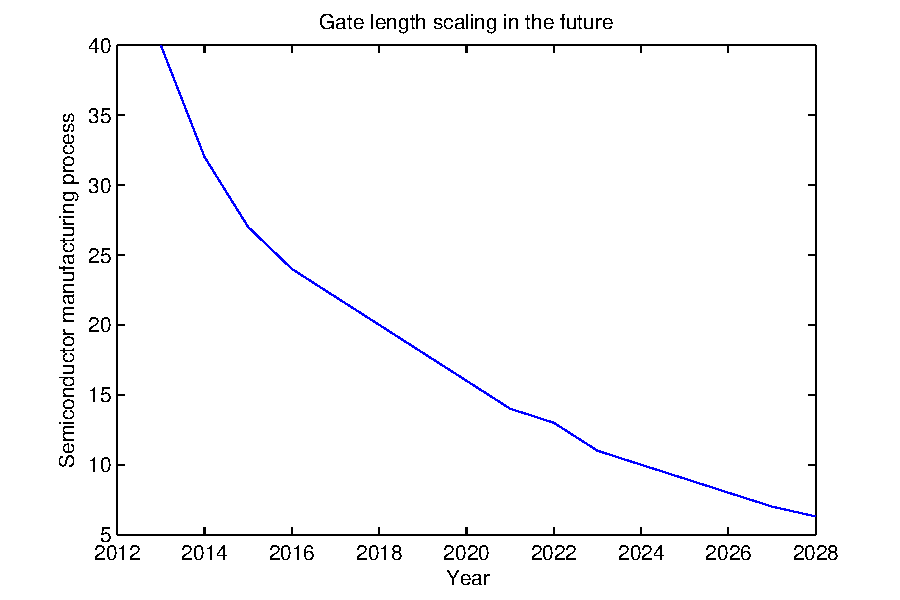
\includegraphics[width = 0.9\textwidth]{E/gate.pdf}
  \caption{Impact of technology scaling into gate length}
 \label{fig:gateE}
 \end{figure}
 
The memory banks consist of the memory cells, which in our case are built using gates.
Thus, the predictions about the future behavior of the memory banks are based on the ITRS reports for logic.
The reports for logic are chosen, because the clustered memory architectures that are studied in this work are synthesized using standard cells.
Different predictions and reports are provided by ITRS for other types of memories, such as DRAM.
However, the proposed scratchpad memory architectures are the preferred choice for our scope.
Typically the memories used in embedded systems are smaller and more energy efficient than DRAM.

In the coming years, the transistor gate length is expected to be reduced as shown in Fig. \ref{fig:gateE} generated from data found in \cite{itrs2}.
The values are approaching 5nm around 2028, which is potentially the limit using the current manufacturing process.
The reduction in gate lengths leads to a reduced size of the memory cell and consequently smaller memory banks.
The smaller memory banks affect both the area of the design and the power consumption.
The projections provided by ITRS regarding the power are presented in Fig. \ref{fig:powerE} generated from data found in \cite{itrs2}. 
There is a significant reduction in power consumption in the short term and slighter reduction towards the end of the projections.

  \begin{figure}
 \centering
 \includegraphics[width = 0.9\textwidth]{E/cellpower.pdf}
  \caption{Memory Banks: Normalized dynamic power and technology scaling}
 \label{fig:powerE}
 \end{figure}

\subsection{Interconnection}

The interconnection cost is based on the projections about wiring, which are different from the projections for logic gates.
The current study is restricted to the reports about the lower and intermediate metal layers, because these are the ones that are relevant for the interconnection of our memory organizations.
The reports about the global interconnection scaling is not our focus, as it is used for the power and clock routing and between computing clusters on large SoC platforms.
However, the changes in size of the memory banks affects the length of the needed wires.
The most important parameters for the current study are the capacitance and the power consumption of the interconnection.
Curves for these two parameters are presented in Fig. \ref{fig:intpowerE} generated from data provided by ITRS \cite{itrs2}.
The capacitance is expected to be reduced in the following year.
Although the capacitance is reduced, the rate of this reduction is lower compared to the expected reduction for the memory cells.
The power values are per length unit and they are expected to rise due to several challenges that the interconnection technology will face in the future.

 \begin{figure}
 \centering
 \includegraphics[width =0.9\textwidth]{E/intpower.pdf}
  \caption{Interconnection: Impact of technology scaling on the capacitance and the power consumption of the interconnection part}
 \label{fig:intpowerE}
 \end{figure}
 
The significant parameter in this work is the capacitance.
Resistance is also generally studied in the interconnection because of its important impact, especially for signal
delay. 
The current work focus on energy rather than delay and this is a rational choice for embedded systems.
In general, the clock speeds are relatively low for a typical embedded system in contrast to high performance computing.
In our target domain, a system architecture includes several processing cores that can be of different types to fulfill different application requirements.
When higher performance is needed in an embedded system, it is usually achieved by adding another processing core or a special hardware unit rather than having an extremely high clock speed.
Thus, it is expected that the critical path delay is not the main worry for a system designer.
If the aim is high-performance designs, the current work has to be extended in the future.
A different approach where delay-energy trade-offs are incorporated
from the start should be developed in such a case. The interconnect resistance would then be important in addition to the capacitance.

\section{Model Construction and Projection Results}
\label{resultsE}

\subsection{Model Construction}

 The scope is to develop a model that can provide a sufficiently accurate estimate of the power overhead for the interconnection in clustered memory architectures.
 The model is based on synthesis results of feasible designs in current technologies and study of the projections provided by ITRS.
 The model focuses on the dynamic power, which is the dominant factor for data intensive applications.
 Although leakage power is increasing for smaller technology nodes, the effect on the proposed clustered architecture is low.
 The main reason is that the part of the memory that is active at a given time is heavily accessed for the target applications, thus the static power is negligible compared to the static power.
 The part of the memory that is not accessed at a given time is normally switched off, thus the static power is heavily reduced. 
 The study of the dynamic power is hence sufficient within our scope.
 The interconnect static power is generally low compared to the memory banks as discussed in \cite{liu1994power}.
 
 The input for the model is the process technology and the configuration of the clustered memory architecture.
 The process technology leads to different points in Fig. \ref{fig:powerE} and Fig. \ref{fig:intpowerE} for the memory banks and the interconnection respectively.
 For the ITRS predicted year of a given technology on the x-axis chosen, the corresponding normalized values for dynamic memory power, interconnect capacitance and power can be found. 
 The configuration of the architecture reveals the number of memory banks and all widths and lengths of the memory configuration.
 The power consumed by the memory banks is calculated using the total number of memory cells:
 \begin{center}
 $$ Banks_{power} \propto \sum_{Banks}^{for all} W \times L \times Cell_{power} $$
 \end{center}
  where $W$ and $L$ is the width and the length of each memory bank measured in memory cells. 
  The power per cell is extracted using Fig. \ref{fig:powerE}.
  Each technology node year on the x-axis, leads to the corresponding cell power on the y-axis.

  
 The prediction of the power consumption on the interconnection logic is based in Fig. \ref{fig:intpowerE} in a similar way.
 Based on the technology and the number of memory banks, the length of the wires is calculated, which again gives the power and the capacitance.
 The general formula for the power consumption on a wire is:  
 \begin{center}
 $Power = \dfrac{1}{2} \times f \times C \times V^{2} $
 \end{center}
 where  $f$ is the activity factor, $C$ the capacitance and $V$ the supply voltage.
 However, the simulation results and the projections provided by ITRS suggest that a more detailed model is needed. 
 The basic principle for the model is that the overall interconnection power is proportional to the power of the wires and their capacitance, as explained in  the model presented in \cite{wong2000modeling} and justified on the interconnection study in \cite{muralimanohar2007interconnect}.
 Thus, the general formula for the interconnection power is:
 \begin{center}
 $$ Interconnection_{power} \propto Area(W,L) \times Wire_{power} \times Capacitance $$
 \end{center}
 where $Area$ is calculated based on the total width and length of the memory banks according to the selected configuration.
  In more detail, the different memory banks are placed in a structure similarly to the configuration presented in Fig. \ref{fig:platformE}.
  The library of memory banks provides all the necessary information regarding their sizes.
  The simulation results for the synthesized configurations provide a sufficiently accurate estimate of the area needed for the interconnection, given the number and the sizes of the memory banks.
 The model for the interconnection power cost overhead for a given target technology $ t $ is given by the $ Banks_{power}$ and the $ Interconnection_{power}$:
 \begin{center}
 $$ Overhead = \dfrac{Area(W,L) \times Wire_{power}(t) \times Capacitance(t)}{\sum_{Banks}^{for all} W \times L \times Cell_{power}(t)} $$ 
  \end{center}
 where 
 \begin{itemize}
 \item $ Wire_{power}(t) $ is the wiring efficiency factor based on the power curve in Fig. \ref{fig:intpowerE}
 \item $Capacitance(t)$ is the capacitance of the interconnection wires for the given technology and the length of wiring based on the area, which is calculated for the different number of banks
 \item $Cell_{power} $ is the power consumption of a memory bank for the given technology
 \end{itemize}
 The model is an approximation of the interconnection overhead and the goal is to produce results for relative comparison. 

 The development of the interconnection cost overhead using the proposed model is presented in Fig. \ref{fig:overheadE}.
 The interconnection overhead is kept below 10\% for most of the cases.
 It exceeds this limit in designs with 5 memory banks around a decade from now.
 As expected, the overhead increases as we move from 2 towards 5 memory banks.
 However, the increase is much higher between a design of 4 and 5 memory banks compared to the smaller configurations.
 As motivated before, a memory architecture with six banks is not presented due to the expected high overhead that cannot be justified with the reconfiguration energy gains.
 The interconnection overhead predicted by the model is compared with the synthesis results for the current technology.
 In Tab. \ref{tab:verification} the first column is the overhead percentage presented in Tab. \ref{tab:overhead} and the second column the predicted overhead percentage presented in Fig. \ref{fig:overheadE}.
 The agreement between the two suggests that the model is sufficiently accurate for the current technology.
 
 \begin{center}
	\begin{table}
	\caption{Comparison between predicted and simulated overhead}
	\label{tab:verification}
	\centering
	{
	\begin{tabular}{|c|c|c|}
	\hline
	Number of Banks &	Simulated Overhead & Predicted Overhead \\
	\hline
	2 & 1.26\%  & 1.16\% \\
	\hline 
	3 & 1.37\%  & 1.26\% \\
	\hline 
	4 & 1.77\% & 1.63\% \\
	\hline
	5 & 3.0\% & 2.78\% \\
	\hline	
	\end{tabular}}
	\end{table}
\end{center}

 \begin{figure}
 \centering
 \includegraphics[width = 0.9\textwidth]{E/overhead.pdf}
  \caption{Projections of the interconnection cost power overhead for different numbers of memory banks}
 \label{fig:overheadE}
 \end{figure} 

 
\subsection{Results}
 
The model is useful during exploration of efficient clustered memory organization for a given application and technology. 
Based on Fig. \ref{fig:overheadE} it is likely that the optimum memory organization for a 45 nm design will include more memory banks compared to a 5 nm design.
The overall results also indicates that since the overhead is small, the design approach using clustered memory architectures will be relevant in the future.
The model provides necessary information to the system designer and steers the decision about the number of banks in the memory architecture for a given technology.
The improvement in the designer's decision is a strong motivation for the development of the model. 

To better illustrate the change in the optimum memory architecture for future technologies, an example application is chosen.
The EPIC (Efficient Pyramid Image Coder) \nomenclature{EPIC}{efficient pyramid image coder} is an image compression algorithm and its behavior on a clustered image architecture is presented in \cite{filippopoulos2013exploration}.
The energy gains for the most energy efficient memory organizations are presented in Tab. \ref{tab:GainvsOverhead}. In these numbers the cost of the added interconnect is not included.
The energy gain percentage is constant and independent of the technology, because the comparison is always between a monolithic and a clustered memory architecture of the same technology.
The sizes of the memory banks for each configuration are used to calculate the interconnection overhead for synthesizing in 45nm and 5nm.
The percentage of the energy overhead due to the interconnection cost is also presented in Tab. \ref{tab:GainvsOverhead} both for the current and the most advanced technology.
Based on the improvements and the overheads the most energy efficient design for a specific technology can be defined for the EPIC benchmark application.
For the 45nm technology, a clustered memory architecture with five memory banks is the optimum, while for the 5nm technology four memory banks give the optimal solution.
The addition of a fifth bank reduces the energy consumption by 2.7\%, as a result of the lower energy consumption inside the memory banks, but at the same time increases the energy consumption by 4.5\%, as a result of the higher energy consumption on the interconnection between the banks.

\begin{center}
	\begin{table}
	\centering
	\caption{Energy gains vs. interconnection overhead}
	\label{tab:GainvsOverhead}
	{
	\begin{tabular}{|c|c|c|c|c|}
	\hline
	Banks & Sizes [kB] & Gains & Overhead(45nm) & Overhead(5nm) \\
	\hline
	2 & 8/32 & 40.1\%   & 0.8\%  & 4.6\%  \\
	\hline 
	3 & 8/8/16 & 47.6\%   & 0.9\%  & 4.9\% \\
	\hline 
	4 & 8/8/8/8 & 51.7\% & 1.2\% & 6.4\% \\
	\hline
	5 & 2/8/8/8/8 & 54.4\% & 2.0\% & 10.9\% \\
	\hline	
	\end{tabular}}
	\end{table}
\end{center}
  
\section{Conclusion}
\label{conclusionE}

We have proposed a model that can provide estimates of the interconnection overhead in a clustered memory architecture in future technology nodes.
The model suggests that overhead will be kept low in the short term and will increase within reasonable levels in the mid-long term.
Therefore, the design of energy efficient clustered memory architecture will continue to be a good design choice.
The estimations for the future can be useful for system designers that try to design power efficient architectures for applications with dynamic memory requirements throughout their lifetime.
Another contribution of the model is that it provides an early indication about the optimal number of banks for a given technology and design.
This information reduces the design space exploration and the design time. 
When newer technologies become available in the CAD tools, the designs can be re-synthesized and the model can be calibrated.

%\addcontentsline{toc}{section}{Bibliography}	
%\bibliographystyle{plain}
%\bibliography{reference}

%\end{document}
